\documentclass[dvipdfmx,twoside]{jsarticle}
\usepackage{amsmath,amssymb}
\usepackage{CJKutf8}
\usepackage{okumacro}
\usepackage{booktabs}
\usepackage{array}
\usepackage{xcolor}
\usepackage{colortbl}
\usepackage{tipa}
\usepackage{tikz}
\usepackage{fancybox}
\usepackage{wasysym}
\usepackage{pifont}
\usepackage{graphicx}
\usepackage{wrapfig}
\usepackage{geometry}
\geometry{margin=2cm}
\usepackage{fancyhdr}
\usepackage[utf8]{inputenc}
\usepackage{CJK}
% 设置页面样式
\pagestyle{fancy}
\fancyhf{}
\renewcommand{\headrulewidth}{0pt}
\fancyhead[RO]{数学–\thepage}
\fancyhead[LE]{数学–\thepage}

% 重新定义 plain 样式
\fancypagestyle{plain}{%
  \fancyhf{}%
  \renewcommand{\headrulewidth}{0pt}%
  \fancyhead[RO]{数学-\thepage}%
  \fancyhead[LE]{数学-\thepage}%
}
% 自定义A方框命令
\newcommand{\abb}[1]{%
\begin{tikzpicture}[baseline]
\node[draw=black, 
      rectangle, 
      minimum width=0.8cm, 
      minimum height=0.3cm, 
      fill=gray!25, 
      font=\bfseries,
      line width=1pt,
      inner sep=2pt,
      anchor=base] {#1};
\end{tikzpicture}%
}
\newcommand{\ab}[1]{%
\begin{tikzpicture}[baseline]
\node[draw=black, 
      rectangle, 
      minimum width=0.8cm, 
      minimum height=0.3cm, 
      font=\bfseries,
      line width=1pt,
      inner sep=2pt,
      anchor=base] {#1};
\end{tikzpicture}%
}

\newcommand{\maru}[1]{\tikz[baseline=-0.7ex]{
    \node[shape=circle,draw,inner sep=1pt,minimum size=5pt,anchor=center] {\footnotesize #1};}}
\definecolor{headercolor}{RGB}{220,220,220}
\definecolor{rowcolor1}{RGB}{245,245,245}
\definecolor{rowcolor2}{RGB}{255,255,255}

% \title{\vspace{-1.5cm} 2025年8月羚課文科数学月考 }
% \author{\textnosfal{Linc\ -\ 伊}}
\date{}
\begin{document}

\begin{CJK}{UTF8}{ipxm}  % 使用ipxm字体
  %月考表纸部分
\begin{center}

\vspace*{5cm}

% 学校logo

\includegraphics[width=5cm]{pics/1.jpg}

\vspace{2cm}

% 主标题
{\fontsize{24}{30}\selectfont\bfseries\sffamily
2025年8月\\
\vspace{1em}
羚課文科数学月考
}

\end{center}
\newpage
%第一部分
\noindent
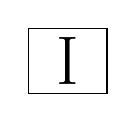
\begin{tikzpicture}
\node[draw, rectangle, minimum width=1cm, minimum height=0.8cm, font=\Huge] {I};
\end{tikzpicture}
\\
\\


\end{document}